%  A simple AAU report template.
%  2015-05-08 v. 1.2.0
%  Copyright 2010-2015 by Jesper Kjær Nielsen <jkn@es.aau.dk>
%
%  This is free software: you can redistribute it and/or modify
%  it under the terms of the GNU General Public License as published by
%  the Free Software Foundation, either version 3 of the License, or
%  (at your option) any later version.
%
%  This is distributed in the hope that it will be useful,
%  but WITHOUT ANY WARRANTY; without even the implied warranty of
%  MERCHANTABILITY or FITNESS FOR A PARTICULAR PURPOSE.  See the
%  GNU General Public License for more details.
%
%  You can find the GNU General Public License at <http://www.gnu.org/licenses/>.
%
%  A simple AAU report template.
%  2015-05-08 v. 1.2.0
%  Copyright 2010-2015 by Jesper Kjær Nielsen <jkn@es.aau.dk>
%
%  This is free software: you can redistribute it and/or modify
%  it under the terms of the GNU General Public License as published by
%  the Free Software Foundation, either version 3 of the License, or
%  (at your option) any later version.
%
%  This is distributed in the hope that it will be useful,
%  but WITHOUT ANY WARRANTY; without even the implied warranty of
%  MERCHANTABILITY or FITNESS FOR A PARTICULAR PURPOSE.  See the
%  GNU General Public License for more details.
%
%  You can find the GNU General Public License at <http://www.gnu.org/licenses/>.
%
\documentclass[11pt,twoside,a4paper,openright]{report}
%%%%%%%%%%%%%%%%%%%%%%%%%%%%%%%%%%%%%%%%%%%%%%%%
% Language, Encoding and Fonts
% http://en.wikibooks.org/wiki/LaTeX/Internationalization
%%%%%%%%%%%%%%%%%%%%%%%%%%%%%%%%%%%%%%%%%%%%%%%%
% Select encoding of your inputs. Depends on
% your operating system and its default input
% encoding. Typically, you should use
%   Linux  : utf8 (most modern Linux distributions)
%            latin1 
%   Windows: ansinew
%            latin1 (works in most cases)
%   Mac    : applemac
% Notice that you can manually change the input
% encoding of your files by selecting "save as"
% an select the desired input encoding. 
\usepackage[utf8]{inputenc}
% Make latex understand and use the typographic
% rules of the language used in the document.
\usepackage[danish,english]{babel}
% Use the palatino font
\usepackage[sc]{mathpazo}
\linespread{1.05}         % Palatino needs more leading (space between lines)
% Choose the font encoding
\usepackage[T1]{fontenc}
%%%%%%%%%%%%%%%%%%%%%%%%%%%%%%%%%%%%%%%%%%%%%%%%
% Graphics and Tables
% http://en.wikibooks.org/wiki/LaTeX/Importing_Graphics
% http://en.wikibooks.org/wiki/LaTeX/Tables
% http://en.wikibooks.org/wiki/LaTeX/Colors
%%%%%%%%%%%%%%%%%%%%%%%%%%%%%%%%%%%%%%%%%%%%%%%%
% load a colour package
\usepackage{xcolor}
\definecolor{aaublue}{RGB}{33,26,82}% dark blue
% The standard graphics inclusion package
\usepackage{graphicx}
% Set up how figure and table captions are displayed
\usepackage{caption}
\captionsetup{%
  font=footnotesize,% set font size to footnotesize
  labelfont=bf % bold label (e.g., Figure 3.2) font
}
% Make the standard latex tables look so much better
\usepackage{array,booktabs}
% Enable the use of frames around, e.g., theorems
% The framed package is used in the example environment
\usepackage{framed}

%%%%%%%%%%%%%%%%%%%%%%%%%%%%%%%%%%%%%%%%%%%%%%%%
% Mathematics
% http://en.wikibooks.org/wiki/LaTeX/Mathematics
%%%%%%%%%%%%%%%%%%%%%%%%%%%%%%%%%%%%%%%%%%%%%%%%
% Defines new environments such as equation,
% align and split 
\usepackage{amsmath}
% Adds new math symbols
\usepackage{amssymb}
% Use theorems in your document
% The ntheorem package is also used for the example environment
% When using thmmarks, amsmath must be an option as well. Otherwise \eqref doesn't work anymore.
\usepackage[framed,amsmath,thmmarks]{ntheorem}

%%%%%%%%%%%%%%%%%%%%%%%%%%%%%%%%%%%%%%%%%%%%%%%%
% Page Layout
% http://en.wikibooks.org/wiki/LaTeX/Page_Layout
%%%%%%%%%%%%%%%%%%%%%%%%%%%%%%%%%%%%%%%%%%%%%%%%
% Change margins, papersize, etc of the document
\usepackage[
  inner=28mm,% left margin on an odd page
  outer=41mm,% right margin on an odd page
  %top=,
  %bottom=,
  ]{geometry}
% Modify how \chapter, \section, etc. look
% The titlesec package is very configureable
\usepackage{titlesec}
\titleformat{\chapter}[display]{\normalfont\huge\bfseries}{\chaptertitlename\ \thechapter}{20pt}{\Huge}
\titleformat*{\section}{\normalfont\Large\bfseries}
\titleformat*{\subsection}{\normalfont\large\bfseries}
\titleformat*{\subsubsection}{\normalfont\normalsize\bfseries}
%\titleformat*{\paragraph}{\normalfont\normalsize\bfseries}
%\titleformat*{\subparagraph}{\normalfont\normalsize\bfseries}

% Clear empty pages between chapters
\let\origdoublepage\cleardoublepage
\newcommand{\clearemptydoublepage}{%
  \clearpage
  {\pagestyle{empty}\origdoublepage}%
}
\let\cleardoublepage\clearemptydoublepage

% Change the headers and footers
\usepackage{fancyhdr}
\pagestyle{fancy}
\fancyhf{} %delete everything
\renewcommand{\headrulewidth}{0pt} %remove the horizontal line in the header
\fancyhead[RE]{\small\nouppercase\leftmark} %even page - chapter title
\fancyhead[LO]{\small\nouppercase\rightmark} %uneven page - section title
\fancyhead[LE,RO]{\thepage} %page number on all pages, header
% \fancyfoot[LE,RO]{Page \thepage\space of \pageref{LastPage}} %page number on all pages, footer
% Do not stretch the content of a page. Instead,
% insert white space at the bottom of the page
\raggedbottom
% Enable arithmetics with length. Useful when
% typesetting the layout.
\usepackage{calc}

%%%%%%%%%%%%%%%%%%%%%%%%%%%%%%%%%%%%%%%%%%%%%%%%
% Bibliography
% http://en.wikibooks.org/wiki/LaTeX/Bibliography_Management
%%%%%%%%%%%%%%%%%%%%%%%%%%%%%%%%%%%%%%%%%%%%%%%%
%\usepackage[backend=biber,
%  bibencoding=utf8,
%  style=numeric,
%  sorting = none,
%  %citestyle=apa,
%  language=danish,
%  ]{biblatex}
%\usepackage{url}


\usepackage[square]{natbib}

\bibliographystyle{unsrtnat} % viser referencers url

\usepackage[hyphens]{url} % url formatering
\usepackage{hyperref}

%\usepackage{babel/polyglossia}
\usepackage{csquotes}

%%%%%%%%%%%%%%%%%%%%%%%%%%%%%%%%%%%%%%%%%%%%%%%%
% Misc
%%%%%%%%%%%%%%%%%%%%%%%%%%%%%%%%%%%%%%%%%%%%%%%%
% Add bibliography and index to the table of
% contents
\usepackage[nottoc]{tocbibind}
% Add the command \pageref{LastPage} which refers to the
% page number of the last page
\usepackage{lastpage}
% Add todo notes in the margin of the document
\usepackage[
%  disable, %turn off todonotes
  colorinlistoftodos, %enable a coloured square in the list of todos
  textwidth=\marginparwidth, %set the width of the todonotes
  textsize=scriptsize, %size of the text in the todonotes
  ]{todonotes}

%%%%%%%%%%%%%%%%%%%%%%%%%%%%%%%%%%%%%%%%%%%%%%%%
% Hyperlinks
% http://en.wikibooks.org/wiki/LaTeX/Hyperlinks
%%%%%%%%%%%%%%%%%%%%%%%%%%%%%%%%%%%%%%%%%%%%%%%%
% Enable hyperlinks and insert info into the pdf
% file. Hypperref should be loaded as one of the 
% last packages
\usepackage{hyperref}
\hypersetup{%
	plainpages=false,%
	pdfauthor={Author(s)},%
	pdftitle={Title},%
	pdfsubject={Subject},%
	bookmarksnumbered=true,%
	colorlinks=false,%
	citecolor=black,%
	filecolor=black,%
	linkcolor=black,% you should probably change this to black before printing
	urlcolor=black,%
	pdfstartview=FitH%
}


% skriv \par for halvt linieskift 
\setlength{\parindent}{0em}    %bestemmer indrykning på linie
\setlength{\parskip}{0.5em}    %bestemmer størrelse af linieskift

\usepackage{float}
\usepackage{booktabs}
\usepackage{enumitem}

\usepackage{amssymb}

\usepackage{longtable}

\usepackage{makecell}

\newlength\mytemplength

\newcommand\parboxc[3]{%
    \settowidth{\mytemplength}{#3}%
    \parbox[#1][#2]{\mytemplength}{\centering #3}%
}


\usepackage{listings}

%Coding:
\usepackage[newfloat]{minted}
\usepackage{caption}
\newenvironment{code}{\captionsetup{type=listing}}{}
\SetupFloatingEnvironment{listing}{name=Code example}

\usepackage{csquotes}

% Viser mere info om fejl
%\setcounter{errorcontextlines}{999}% package inclusion and set up of the document
% see, e.g., http://en.wikibooks.org/wiki/LaTeX/Formatting#Hyphenation
% for more information on word hyphenation
\hyphenation{ex-am-ple hy-phen-a-tion short}
\hyphenation{long la-tex}
% 
%  A simple AAU report template.
%  2015-05-08 v. 1.2.0
%  Copyright 2010-2015 by Jesper Kjær Nielsen <jkn@es.aau.dk>
%
%  This is free software: you can redistribute it and/or modify
%  it under the terms of the GNU General Public License as published by
%  the Free Software Foundation, either version 3 of the License, or
%  (at your option) any later version.
%
%  This is distributed in the hope that it will be useful,
%  but WITHOUT ANY WARRANTY; without even the implied warranty of
%  MERCHANTABILITY or FITNESS FOR A PARTICULAR PURPOSE.  See the
%  GNU General Public License for more details.
%
%  You can find the GNU General Public License at <http://www.gnu.org/licenses/>.
%
%
%
% see, e.g., http://en.wikibooks.org/wiki/LaTeX/Customizing_LaTeX#New_commands
% for more information on how to create macros

\DeclareCaptionType{use_case}[Use Case]
\DeclareCaptionType{actor}[Actor]

%%%%%%%%%%%%%%%%%%%%%%%%%%%%%%%%%%%%%%%%%%%%%%%%
% Macros for the titlepage
%%%%%%%%%%%%%%%%%%%%%%%%%%%%%%%%%%%%%%%%%%%%%%%%
%Creates the aau titlepage
\newcommand{\aautitlepage}[3]{%
  {
    %set up various length
    \ifx\titlepageleftcolumnwidth\undefined
      \newlength{\titlepageleftcolumnwidth}
      \newlength{\titlepagerightcolumnwidth}
    \fi
    \setlength{\titlepageleftcolumnwidth}{0.5\textwidth-\tabcolsep}
    \setlength{\titlepagerightcolumnwidth}{\textwidth-2\tabcolsep-\titlepageleftcolumnwidth}
    %create title page
    \thispagestyle{empty}
    \noindent%
    \begin{tabular}{@{}ll@{}}
      \parbox{\titlepageleftcolumnwidth}{
        \iflanguage{danish}{%
          
\includegraphics[width=\titlepageleftcolumnwidth]{figures/aau_logo_da}
        }{%
          
\includegraphics[width=\titlepageleftcolumnwidth]{figures/aau_logo_en}
        }
      } &
      \parbox{\titlepagerightcolumnwidth}{\raggedleft\sf\small
        #2
      }\bigskip\\
       #1 &
      \parbox[t]{\titlepagerightcolumnwidth}{%
      \textbf{Abstract:}\bigskip\par
        \fbox{\parbox{\titlepagerightcolumnwidth-2\fboxsep-2\fboxrule}{%
          #3
        }}
      }\\
    \end{tabular}
    \vfill
    \iflanguage{danish}{%
      \noindent{\footnotesize\emph{Rapportens indhold er frit tilgængeligt, men offentliggørelse (med kildeangivelse) må kun ske efter aftale med forfatterne.}}
    }{%
      \noindent{\footnotesize\emph{The content of this report is freely available, but publication (with reference) may only be pursued due to agreement with the author.}}
    }
    \clearpage
  }
}

%Create english project info
\newcommand{\englishprojectinfo}[8]{%
  \parbox[t]{\titlepageleftcolumnwidth}{
    \textbf{Title:}\\ #1\bigskip\par
    \textbf{Theme:}\\ #2\bigskip\par
    \textbf{Project Period:}\\ #3\bigskip\par
    \textbf{Project Group:}\\ #4\bigskip\par
    \textbf{Participant(s):}\\ #5\bigskip\par
    \textbf{Supervisor(s):}\\ #6\bigskip\par
    %\textbf{Copies:} #7\bigskip\par
    \textbf{Page Numbers:} \pageref{LastPage}\bigskip\par
    \textbf{Date of Completion:}\\ #8
  }
}

%Create danish project info
\newcommand{\danishprojectinfo}[8]{%
  \parbox[t]{\titlepageleftcolumnwidth}{
    \textbf{Titel:}\\ #1\bigskip\par
    \textbf{Tema:}\\ #2\bigskip\par
    \textbf{Projektperiode:}\\ #3\bigskip\par
    \textbf{Projektgruppe:}\\ #4\bigskip\par
    \textbf{Deltager(e):}\\ #5\bigskip\par
    \textbf{Vejleder(e):}\\ #6\bigskip\par
    \textbf{Oplagstal:} #7\bigskip\par
    \textbf{Sidetal:} \pageref{LastPage}\bigskip\par
    \textbf{Afleveringsdato:}\\ #8
  }
}

%%%%%%%%%%%%%%%%%%%%%%%%%%%%%%%%%%%%%%%%%%%%%%%%
% An example environment
%%%%%%%%%%%%%%%%%%%%%%%%%%%%%%%%%%%%%%%%%%%%%%%%
\theoremheaderfont{\normalfont\bfseries}
\theorembodyfont{\normalfont}
\theoremstyle{break}
\def\theoremframecommand{{\color{gray!50}\vrule width 5pt \hspace{5pt}}}
\newshadedtheorem{exa}{Example}[chapter]
\newenvironment{example}[1]{%
		\begin{exa}[#1]
}{%
		\end{exa}
}
% my new macros

\begin{document}
%frontmatter
\pagestyle{empty} %disable headers and footers
\pagenumbering{roman} %use roman page numbering in the frontmatter
%  A simple AAU report template.
%  2015-05-08 v. 1.2.0
%  Copyright 2010-2015 by Jesper Kjær Nielsen <jkn@es.aau.dk>
%
%  This is free software: you can redistribute it and/or modify
%  it under the terms of the GNU General Public License as published by
%  the Free Software Foundation, either version 3 of the License, or
%  (at your option) any later version.
%
%  This is distributed in the hope that it will be useful,
%  but WITHOUT ANY WARRANTY; without even the implied warranty of
%  MERCHANTABILITY or FITNESS FOR A PARTICULAR PURPOSE.  See the
%  GNU General Public License for more details.
%
%  You can find the GNU General Public License at <http://www.gnu.org/licenses/>.
%
\pdfbookmark[0]{Front page}{label:frontpage}%
\begin{titlepage}
  \addtolength{\hoffset}{0.5\evensidemargin-0.5\oddsidemargin} %set equal margins on the frontpage - remove this line if you want default margins
  \noindent%
  \begin{tabular}{@{}p{\textwidth}@{}}
    \toprule[2pt]
    \midrule
    \vspace{0.2cm}
    \begin{center}
    \Huge{\textbf{
      Asset Management System% insert your title here
    }}
    \end{center}
    \begin{center}
      \Large{
        The development of the Asset Management System% insert your subtitle here
      }
    \end{center}
    \vspace{0.2cm}\\
    \midrule
    \toprule[2pt]
  \end{tabular}
  \vspace{4 cm}
  \begin{center}
    {\large
      P3 Project Paper%Insert document type (e.g., Project Report)
    }\\
    \vspace{0.2cm}
    {\Large
      DS303E19%Insert your group name or real names here
    }
  \end{center}
  \vfill
  \begin{center}
  Aalborg University\\
  Computer Science
  \end{center}
\end{titlepage}
\clearpage

\newgeometry{top=20mm, bottom=20mm}
    \thispagestyle{empty}
{\small
\strut\vfill % push the content to the bottom of the page
\noindent Copyright \copyright{} Aalborg University 2019\par
\vspace{0.2cm}
\noindent Here you can write something about which tools and software you have used for typesetting the document, running simulations and creating figures. If you do not know what to write, either leave this page blank or have a look at the colophon in some of your books.
}
\clearpage


    \pdfbookmark[0]{English title page}{label:titlepage_en}
\aautitlepage{%
  \englishprojectinfo{
    Asset Management System %title
  }{%
    Company Communication %theme
  }{%
    Fall Semester 2019 %project period
  }{%
    DS303E19 % project group
  }{%
    %list of group members
    Alexander Nykjær\\
    Ane Søgaard Jørgensen\\
    Daniel Fly\\ 
    Jakob Sønderby Kristensen\\
    Michelle Volf Terpling\\
    Niels Vistisen\\
    Thomas Lorentzen
  }{%
    %list of supervisors
    Lu Chen
  }{
    
  }{%
    \today % date of completion
  }%
}{%department and address
  \textbf{Computer Science}\\
  Aalborg University\\
  \href{http://www.aau.dk}{http://www.aau.dk}
}{% the abstract
    
\begin{verbatim}
        o                o         
                               o     
          o          O            
                ______    o      
              _/  (   \_        
    _       _/  (       \_   O      
    | \_   _/  (   (    0  \        
    |== \_/  (   (          |      
    |=== _ (   (   (        |       
    |==_/ \_ (   (          |     
    |_/     \_ (   (    \__/    
             \_ (      _/         
               |  |___/          
              /__/               
\end{verbatim}
    
}

\restoregeometry
\cleardoublepage
\pdfbookmark[0]{Contents}{label:contents}
\pagestyle{fancy} %enable headers and footers again
\tableofcontents
\listoftodos \todo[inline] {Fjern den her!} 
\chapter*{Preface\markboth{Preface}{Preface}}\label{ch:preface}
\addcontentsline{toc}{chapter}{Preface}
Here is the preface. You should put your signatures at the end of the preface.

\subsection*{Reading Guide}

\vspace{\baselineskip}\hfill Aalborg University, \today
\vfill\noindent
\vspace{0.5\baselineskip}
\begin{minipage}[b]{0.45\textwidth}
 \centering
 \rule{\textwidth}{0.5pt}\\
  Alexander Nykjær\\
 {\footnotesize <anykjal18@student.aau.dk>}
\end{minipage}
\hfill
\begin{minipage}[b]{0.45\textwidth}
 \centering
 \rule{\textwidth}{0.5pt}\\
  Ane Søgaaard Jørgensen\\
 {\footnotesize <asja18@student.aau.dk>}
\end{minipage}

\vspace{1\baselineskip}
\begin{minipage}[b]{0.45\textwidth}
 \centering
 \rule{\textwidth}{0.5pt}\\
  Daniel Fly\\
 {\footnotesize <dfly18@student.aau.dk>}
\end{minipage}
\hfill
\begin{minipage}[b]{0.45\textwidth}
 \centering
 \rule{\textwidth}{0.5pt}\\
  Jakob Sønderby Kristensen\\
 {\footnotesize <jkr18@student.aau.dk>}
\end{minipage}

\vspace{1\baselineskip}
\begin{minipage}[b]{0.45\textwidth}
 \centering
 \rule{\textwidth}{0.5pt}\\
  Michelle Volf Terpling\\
 {\footnotesize <mterpl18@student.aau.dk>}
\end{minipage}
\hfill
\begin{minipage}[b]{0.45\textwidth}
 \centering
 \rule{\textwidth}{0.5pt}\\
  Niels Vistisen \\
 {\footnotesize <nvisti18@student.aau.dk>}
\end{minipage}

%\vspace{3.5\baselineskip}
% 
\vspace{0.8\baselineskip}
\begin{center}
\begin{minipage}[b]{0.45\textwidth}
 \centering
 \rule{\textwidth}{0.5pt}\\
  Thomas Lorentzen\\
 {\footnotesize <tglo18@student.aau.dk>}
\end{minipage}
\end{center}
\cleardoublepage
%mainmatter
\pagenumbering{arabic} %use arabic page numbering in the mainmatter

%%% The main stuff
\chapter{Introduction}\label{ch:introduction}
As companies expand and acquire a growing number of assets, the desire to keep track of these assets and their condition can also grow \citep{ImportanceOfAM}. Creating an overview of the assets, and keeping this overview up to date, is a major task and one that companies sometimes do not address until the number of assets in their possession has become overwhelming \citep{DoNotIgnoreSAM}. These issues are clear when looking at the growing market of asset management software. The submarket of digital asset managements is estimated to grow from 1.2 billion in 2018, to 6,901 billion by 2024 \citep{MarketGrowth}.
\par
While there are many existing solutions, these are often very extensive and try to accommodate a lot of different use cases by adding more data points to the design \citep{SnipeIT}. This can however lead to the system becoming overwhelming itself. A way of making a solution more suitable for a wide range of companies while still keeping it simple, could be to make it more adaptable \citep{CustomSoftware}. With this approach, the individual company will not be overwhelmed with unneeded User Interface (UI) elements, that are only relevant for a few specific companies.
\par
Focusing on a specific department at a specific company, has limited the magnitude of the project. The collaborator of this project has been the IT department at Aalborg Zoo. Therefore, the specific needs of Aalborg Zoo has been a high priority, as they are considered the customer of the finished product.
\par
Aalborg Zoo is located in the center of Aalborg, and welcomes around 341.000 visitors each year \citep{AalborgZoo}. The zoo has 44 employees with different backgrounds and responsibilities \citep{AalborgZoo}. Because of this, the zoo is divided into multiple departments \citep{PersonaleAZ}. The IT department has multiple responsibilities, including supplying the other departments with computers, walkie talkies, routers, and more (see \autoref{sc:aalborgZoo}). In line with the growth of the zoo and technological advancements, the IT department has come in charge of a lot of different assets. These assets can be loaned out to any employee or department at any point, which can make it hard to keep track of their locations and conditions.
\par
To accommodate this growing task and to ensure an overview of the assets, the IT department has requested an asset management system.

\subsubsection*{Problem statement}
Based on the mentioned issues with existing solutions to the problem, the following problem statement has been formulated and used as the main focus of the project.

\begin{quote}
    \textit{How can a system be designed to be more adaptable than existing asset management systems?}
\end{quote}

% How can a system help Aalborg Zoo manage their assets better than existing tools can?

% How can a system be created to help the IT department at Aalborg Zoo manage their assets?

% How to develop a software system to help the IT department at Aalborg Zoo to manage their systems?

% How can a system, that helps Aalborg Zoo manage their assets, be designed and implemented?

% How can a software solution help manage Aalborg Zoo's assets?


\input{sections/ExistingSolutions.tex}
% Background
\chapter{Aalborg Zoo}\label{ch:problemdefinition}
A series of semi-structured interviews have been conducted with the head of the IT department Morten Rom and technician Kasper Andersen, who make up the IT department at Aalborg Zoo. They describe a problem with keeping track of and maintaining assets within the zoo. Aalborg Zoo covers a large area and assets can be spread around the park. 
\par
Knowing the location of each individual assets comes down to the different employees in the zoo. As a result, no one has a clear picture of the assets within the zoo. Therefore Aalborg Zoo has been looking at different asset management systems. Currently the they do not have the resources to develop such a system for themselves, and has examined other options. However, none of these satisfy their requirements. They want a program that is cheap and easy to use, without presenting the user with a large number of fields to fill out for each new entry into the system. 
%Currently the zoo doesn't have the resources to develop such a system for themselves, and has examined other options. However, none of the systems the zoo has looked at, makes it easy for the user to customize and modify templates.
\par
During the interview process, the head of the IT department expressed a desire for an asset management system with the following requirements. These are presented using the MoSCoW method for prioritization:
\par





%\begin{itemize}
%    \item Make it possible for an administrator to record when employees borrow assets, or associate an asset with a location. This should be done by adding special tags, like a user or location tag.
    
%    \item Add uncategorized tags with additional relevant information to assets. This could be the status of the asset, if for example it is under maintenance. 
    
%    \item A log of the changes made to assets, along with information about who made the change and when it was made. It should also be logged when an asset is added or removed. 
    
%    \item Templates for assets, with only the necessary fields that all assets of that template need to have. For example a switch needs fields with ID, IP-address, and password. All other relevant information can be added through tags.
%\end{itemize}

%The reason for the small number of required fields, is due to the clients wishes. They expressed a dislike for other asset management systems that required too many fields to be filled for each asset. They also wanted as few clicks of the mouse as possible.

\textbf{Must have}:
\begin{enumerate}
    \item Assets can be added, removed, and edited.
    
    \item Tags can be added to the assets. These tags may contain a number of fields. 
    
    \item It will be possible to search through all assets with either ID or name.
    
    \item Information on users will be imported from the Active Directory.
\end{enumerate}

\textbf{Should have}:
\begin{enumerate}
\setcounter{enumi}{4}
    \item Assets and log entries can be exported to a file based on a search.
    
    \item Admins and viewers can add comments to assets. Admins can remove and edit all comments, while viewers can only edit their own comments.
    
    \item Comments for each asset will be accessible from within the specific asset.
    
    \item All changes to assets, tags, and comments will be logged.
    
    \item Field will be set to a certain type and can be marked as required. It will be possible for a field to have a default value. 

    \item The design will be very minimalist.
    
    \item Tags will be presented in different colors. Subtags will inherit the color of their parent tag. Colors will be assigned randomly if not chosen by the user. 
\end{enumerate}

\textbf{Nice to have}:
\begin{enumerate}
\setcounter{enumi}{11}
    \item Departments can be added, removed, and edited. Each user can set their default department.
    
    \item Tags are department specific.
    
    \item It will be possible to select multiple assets or select all and then deselect certain assets. The selected assets can then be exported to a file. 
    
    \item When searching for assets, a list of tags on the found assets will be shown. From this list it will be possible to hide assets by deselecting tags.    
    
    \item Notifications will be based on function tags.\todo{Function tags skal forklares}
    
    \item Viewers can request an asset. The admins can view, approve, or deny all requests for assets. 
\end{enumerate}
    
\textbf{Won't have}:
\begin{enumerate}
\setcounter{enumi}{17}
    \item AND, OR, and parentheses can be used to enable complex searching.
    
    \item System functions can be linked to barcodes. 
\end{enumerate}





\section{Problem Definition}
Based on the interviews with Aalborg Zoo the following problem definition has been formulated:
\begin{quote}
\textit{The IT department at Aalborg Zoo has many assets to keep track of. They currently have no system to help them do so and existing systems do not meet their requirements.}
\end{quote}
For the solution to this problem, a system definition is described in the following section.
\section{System Definition}
The system will be developed to help the IT department at Aalborg Zoo track their corporate assets.
\par
The primary functionality of the system is to give the user the ability to add, edit, remove, and search through all assets. The search will be based on the assets' unique IDs, names, and other identifiers specified by the user, and is limited to the chosen department. When adding a new asset to the system, the user will be able to add predefined tags to the asset. These tags can contain fields that should be filled out for the specific assets.
\par
Secondly, the system will have the functionality to tag assets with their location, the person borrowing the asset, and other attributes. These tags will be usable as identifiers for search queries. The user will be able to add new tags dynamically to the system and assign these to super tags, such as\todo[inline]{Kunne sætningen være: The user will be able to dynamically add tags, and group these using super tags, such as...} 'Locations' or 'Users'. The super tags will act as tag groups, and can also be dynamically added by the user. 
\par
Another secondary functionality of the system is logging activities. The system will be able to provide a history of events for each asset. Events include adding an asset, editing an asset, adding and removing tags on an asset. The user will also be able to attach events performed outside of the system, such as updating the OS of a computer and installing new software to an asset. Every event will have the username of the person who made the change attached.
\par
The system will be used by the IT department, and have a group of users who can manage the system, logging in automatically using their Active Directory (AD) username. All employees will be able to view and comment on the assets, but only the assigned administrators will have the ability to manage them. 
\par
The interface will be simple and easy to use, dynamically changing depending on the department selected. The user will be able to generate a list of assets and export it as a file. The user will also have the ability to dynamically create and edit assets, by adding and removing tags with fields, in order to track specific elements of different assets. It will also be possible to create new tags and attach these to assets dynamically.
\par
The system will be programmed using the C\# language and will be developed for for a Windows PC. The system will be communicating with an MSSQL server and an AD on the internal network. The graphical user interface will be created with the Windows Presentation Foundation (WPF) framework.
\par
The objects in the problem domain are: 
\begin{itemize}
    \item \textbf{Asset}: Corporate assets in Aalborg Zoo, such as a computer, a switch, a phone, etc.

    \item \textbf{Department}: The different departments within Aalborg Zoo, such as finance, IT, etc.
    
    \item \textbf{Admin}: Users with access to manage and lend assets to other employees.
    
    \item \textbf{Viewer}: Users with access to the system, but not the ability to change anything.
    
    %\item \textbf{Borrower}: The employees borrowing assets from the IT department.
\end{itemize}

% Problem domain analysis
\chapter{Problem Domain Analysis}\label{ch:problemdomain}


\section{Classes} \label{sc:classes}
The interviews with the client, made it possible to define the objects in the problem domain, and the relationships between them. This is illustrated in a class diagram (figure \ref{fig:ClassDiagram}).

% Figur af klassediagrammet
\begin{figure}[H]
    \centering
    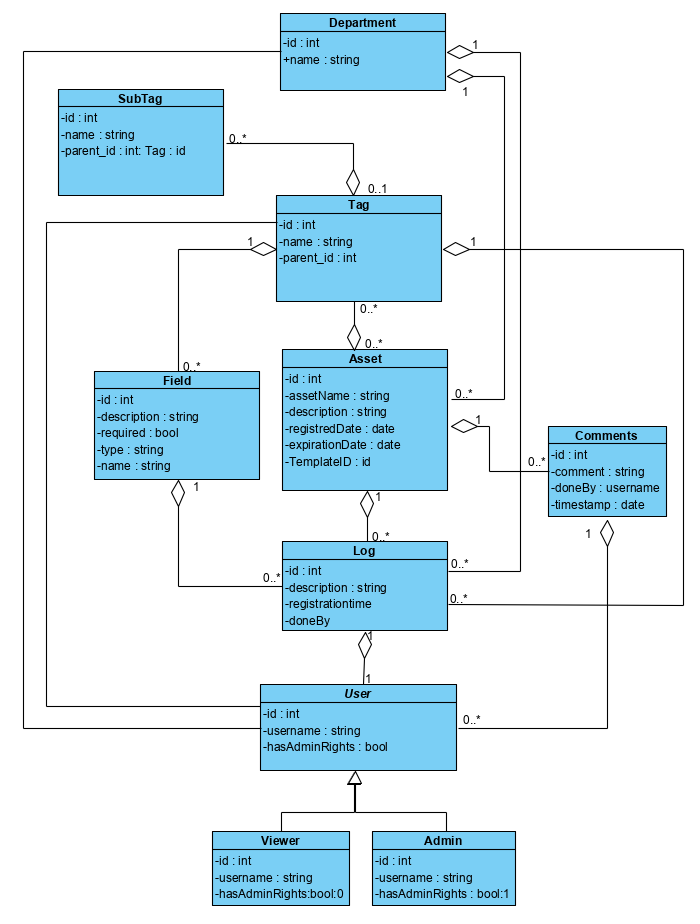
\includegraphics[width=1.0\textwidth]{figures/ClassDiagramV3.png}
    \caption{Class diagram of the objects in the problem domain.}
    \label{fig:ClassDiagram}
\end{figure}

% Beskriv den overordnede ide med systemet ud fra klassediagrammet?

% In figure \ref{fig:ClassDiagram} the connections between a number of classes is shown. These classes are describes as such: \par

The system is developed to support assets with different \textit{tags} attached. An \textit{asset} is, in the context of this project, understood as any physical item, or license belonging to a \textit{department}. A \textit{department} represents a department at the Zoo, and is implemented to function as a group of \textit{assets}, so a user can search for \textit{assets} in a specific \textit{department}.
\par
\textit{tag} is an identifier, which makes it possible to group assets. An \textit{Asset} contains zero or more tags and a \textit{tag} can be attached to zero or more \textit{assets}. This depicts a many-to-many relation between the two classes, which enables multiple assets with the same tag, and multiple tags attached to the same asset. A \textit{tag} can add a number of \textit{fields} to the asset it is attached to. These \textit{fields} can then be filled out by the user, providing additional information about the \textit{asset} dynamically. Some \textit{fields} may be required to be filled out.
Tags can be grouped and managed using supertags/subtags. A tag becomes a sub tag, when it has a relation to another tag.
\todo{Subtags/supertags relationen - måske skrevet} 

\subsection{State change diagrams}

\begin{figure}[H]
    \centering
    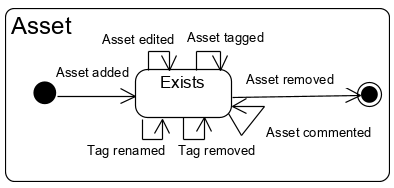
\includegraphics{figures/Asset_statechart.png}
    \caption{Statechart diagram for Asset}
    \label{fig:asset_statechart}
\end{figure}

Throughout the lifetime of an asset it only has a few connected events. After it has been created it can be modified in different ways. 
\begin{itemize}
    \item Asset can be edited, this can include, name changes.
    \item Asset tagged, this links a tag to the asset.
    \item Tag renamed, this gives one of the connected tags a new name.
    \item Tag removed(Asset untagged) this disconnects the link between the asset and a tag.
    \item Asset commented, this event is triggered when a user leaves a comment on the asset.
\end{itemize}
The assets lifetime ends when the asset is removed from the database, and is therefor no longer getting tracked. The statechart for an asset, can be seen on \ref{fig:asset_statechart}.

\begin{figure}[H]
    \centering
    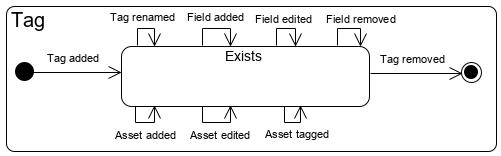
\includegraphics{figures/Tag_statechart.png}
    \caption{Statechart diagram for Tag}
    \label{fig:tag_statechart}
\end{figure}

The lifetime of a tag begins when a tag is added to the system. An existing tag can be affected by several events. For example when changes are made to the tag itself, or associated fields and assets. The lifetime of a tag ends when it is removed from the system. The statechart for the behavior of the tag class, is demonstrated in figure \ref{fig:tag_statechart}.

\begin{figure}[H]
    \centering
    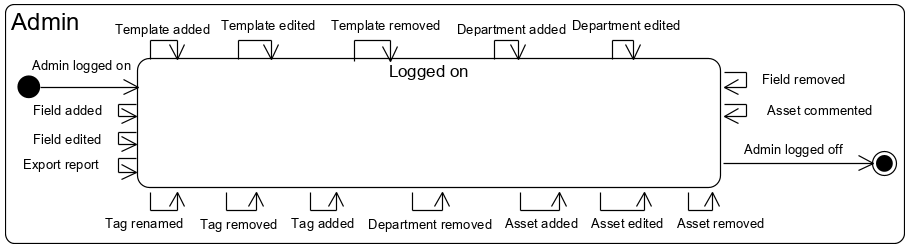
\includegraphics[width=14cm]{figures/Admin_statechart.png}
    \caption{Statechart diagram for Admin}
    \label{fig:admin_statechart}
\end{figure}

The admin class has a larger number of possible events, as this is a user with privileges to make changes in the system. An admin object is created when a user with administrator privileges logs in to the system. Then it is possible to add or remove objects, or edit those that are already present in the system. For example it is possible to add, remove, or edit tags on a particular asset, or comment on an asset. It is also possible for an admin to get a log of all the changes that has been made in the system. An administrator object is terminated when the user with administrator privileges logs off the system. This behavior is illustrated in figure \ref{fig:admin_statechart}.

\begin{figure}[H]
    \centering
    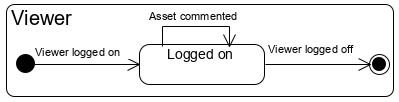
\includegraphics{figures/Viewer_statechart.png}
    \caption{Statechart diagram for Viewer}
    \label{fig:viewer_statechart}
\end{figure}

\begin{figure}[H]
    \centering
    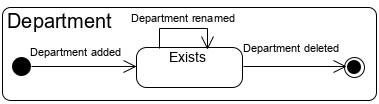
\includegraphics{figures/Department_statechart.png}
    \caption{Statechart diagram for Department}
    \label{fig:department_statechart}
\end{figure}

\begin{figure}[H]
    \centering
    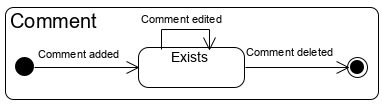
\includegraphics{figures/Comment_statechart.png}
    \caption{Statechart diagram for Comment}
    \label{fig:comment_statechart}
\end{figure}

\begin{figure}[H]
    \centering
    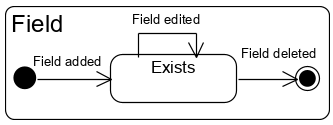
\includegraphics{figures/Field_statechart.png}
    \caption{Statechart diagram for Field}
    \label{fig:field_statechart}
\end{figure}

The classes Viewer, Department, Comment and Field all have similar behavior. As figures \ref{fig:viewer_statechart}, \ref{fig:department_statechart}, \ref{fig:comment_statechart} and \ref{fig:field_statechart} show, the objects are created either when they are added by an admin, or in the case of a Viewer, when a user without administrator privileges logs in. Then the only possible event is the editing of the object. The objects are terminated when they are removed from the system, or when they log off in the case of a Viewer.
\section{Events}\label{sc:events}

In the system the classes, described in section \ref{sc:classes}, interact with each other and the system model. These interactions can be described by events. An event table (table \ref{tab:events}) has been set up to illustrate the connections between classes and events. 

\begin{table}[H]
\centering
\resizebox{\textwidth}{!}{%
    \begin{tabular}{|l||c|c|c|c|c|c|c|c|c|}
        \hline
        & Asset & Department & Admin & Viewer & Log & Tag & Subtag & Field & Comment \\
        \hline
        \hline
        Asset Added & + & & * & & * & & & & \\
        \hline
        Asset removed & + & & * & & * & & & & \\
        \hline
        Asset edited & * & & * & & * & * & * & & \\
        \hline
        Asset tagged & * & & * & & * & * & * & & \\
        \hline
        \hline
        Department added & & + & * & & * & & & & \\
        \hline
        Department removed & & + & * & & * & & & & \\
        \hline
        Department edited & & * & * & & * & & & & \\
        \hline
        \hline
        Tag added & & & * & & * & + & & & \\
        \hline
        Tag removed & & & * & & * & + & & & \\
        \hline
        Tag renamed & & & * & & * & * & * & & \\
        \hline
        Subtag added & & & * & & * & + & + & & \\
        \hline
        Subtag removed & & & * & & * & + & + & & \\
        \hline
        Field added & & & * & & * & * & & + & \\
        \hline
        Field removed & & & * & & * & * & & + & \\
        \hline
        Filed edited & & & * & & * & * & & * & \\
        \hline
        \hline
        Viewer allowed access & & & & * & * & & & & \\
        \hline
        Viewer denied access & & & & * & * & & & & \\
        \hline
        Viewer loggen on & & & & * & * & & & & \\
        \hline
        Viewer logged off & & & & * & * & & & & \\
        \hline
        \hline
        Admin allowed access & & & * & & * & & & & \\
        \hline
        Admin denied access & & & * & & * & & & & \\
        \hline
        Admin logged on & & & * & & * & & & & \\
        \hline
        Admin logged off & & & * & & * & & & & \\
        \hline
        \hline
        Comment added & * & & * & * & * & & & & + \\
        \hline
        Comment removed & * & & * & * & * & & & & * \\
        \hline
        Comment edited & * & & * & * & * & & & & + \\
        \hline
    \end{tabular}
}
\caption{Event table showing which classes are involved with the different events. An event can happen one (+) or several (*) times for each class.}\label{tab:events}
\end{table}


% Application Domain Analysis
\chapter{Application Domain Analysis} \label{ch:applicationdomain}

\section{Actors}\label{sc:actors}

The system will be used by two different types of actors, \textit{Admins} and \textit{Viewers}. These are described as follows:

\begin{actor}[H]
    \hrule
    \vskip 0.3cm
    \Large
    \begin{center}
        \textbf{Admin}
    \end{center}
    \vskip 0.1cm
    \hrule
    \vskip 0.2cm
    \normalsize
    
    \textbf{Goal:} The \textit{admin} manages the system. The \textit{admin's} basic need is to keep track of their assets.
    
    \vskip 0.2cm
    
    \textbf{Characteristics:} The \textit{admin} is the primary user of the system, and is the only person who can change anything regarding the assets in the system. They are experienced with using the system.
    
    \vskip 0.2cm
    
    \textbf{Examples:} \textit{Admin A} is used to organising large quantities of assets, and sees the asset management system as a supplement to their organisational tools.
    \vskip 0.1cm
    \textit{Admin B} is new to asset management, and needs a tool that can help them in all aspects of organising.
    
    \vskip 0.4cm
    \hrule
    \vskip 0.2cm
    \caption{Adding an asset} \label{actor:admin}
\end{actor}


\begin{actor}[H]
    \hrule
    \vskip 0.3cm
    \Large
    \begin{center}
        \textbf{Viewer}
    \end{center}
    \vskip 0.1cm
    \hrule
    \vskip 0.2cm
    \normalsize
    
    \textbf{Goal:} The \textit{viewer} can observe the system's contents. Their need is to get an overview of the status of different assets that might be relevant for their work. 
    
    \vskip 0.2cm
    
    \textbf{Characteristics:} The \textit{viewer} is the secondary user of the system. They can only comment on assets in the system. They have varying degrees of technical competence.
    
    \vskip 0.2cm
    
    \textbf{Examples:} \textit{Viewer A} is familiar with computer systems and has no trouble finding their way around the asset management system.
    \vskip 0.1cm
    \textit{Viewer B} is less experienced with computer systems and is more comfortable talking directly to the admin instead of using the system themselves. 
    
    \vskip 0.4cm
    \hrule
    \vskip 0.2cm
    \caption{Adding an asset} \label{actor:viewer}
\end{actor}


\section{Use cases}\label{sc:usecases}
This section will describe use cases, which will help develop a system that solves the problems and fulfills the needs of the customer.

\begin{use_case}[H]
    \hrule
    \vskip 0.3cm
    \Large
    \begin{center}
    
        \textbf{Adding an asset}
        
    \end{center}
    \vskip 0.1cm
    \hrule
    \vskip 0.2cm
    \normalsize
    
    \textbf{Use Case:} Adding an \textit{asset} to the system is initiated by an \textit{admin}, when he/she goes to the 'add asset' page by pressing 'add new asset' on the 'asset' page. The \textit{admin} tags the \textit{asset} with the desired \textit{tags} and the associated \textit{fields} are presented to him/her in a column next to the list of added \textit{tags}. The \textit{admin} can add and remove \textit{tags} throughout the process and the \textit{fields} will appear and disappear respectively. The \textit{admin} then fills out the presented \textit{fields} and presses 'Add' or 'CTRL + ENTER' to add the \textit{asset} to the database, ending the use case.
    
    \vskip 0.2cm
    
    \textbf{Objects:} Admin, Asset, Tag, Field, Log
    
    \vskip 0.2cm
    
    \textbf{Functions:} Add asset, Tag asset, Untag asset
    
    \vskip 0.4cm
    \hrule
    \vskip 0.2cm
    \caption{Adding an asset} \label{use_case:adding_an_asset}
\end{use_case}

%%%%%%%%%%%%%%%%%%%%%%%%%%%%%%%%%%%%%%

\begin{use_case}[H]
    \hrule
    \vskip 0.3cm
    \Large
    \begin{center}
    
        \textbf{Editing an asset}
        
    \end{center}
    \vskip 0.1cm
    \hrule
    \vskip 0.2cm
    \normalsize
    
    \textbf{Use Case:} An \textit{admin} initiates editing of an \textit{asset} by going to the page for a specific \textit{asset} and pressing the 'edit' button. The \textit{admin} is then taken to a page very similar to the 'add asset' page, where the field and tags of the \textit{asset} are shown as if the \textit{asset} was being added. Here the \textit{admin} can change the values of the fields, add tags and remove tags. When the \textit{asset} has been modified, he \textit{admin} presses 'save', saving the changes and ending the use case.
    
    \vskip 0.2cm
    
    \textbf{Objects:} Admin, Asset, Tag, Field, Log
    
    \vskip 0.2cm
    
    \textbf{Functions:} Edit asset
    
    \vskip 0.4cm
    \hrule
    \vskip 0.2cm
    \caption{Editing an Asset} \label{use_case:edit_asset}
\end{use_case}

%%%%%%%%%%%%%%%%%%%%%%%%%%%%%%%%%%%%%%

\begin{use_case}[H]
    \hrule
    \vskip 0.3cm
    \Large
    \begin{center}
    
        \textbf{Removing an asset}
        
    \end{center}
    \vskip 0.1cm
    \hrule
    \vskip 0.2cm
    \normalsize
    
    \textbf{Use Case:} An \textit{asset} can be removed from the page of the specific asset. On the page for the \textit{asset}, a dropdown in the top-right uncovers a button for deleting the \textit{asset}. When the button is pressed, the \textit{admin} is prompted with a confirmation and, if accepted, the \textit{asset} is removed from the system.
    
    \vskip 0.2cm
    
    \textbf{Objects:} Admin, Asset, Log
    
    \vskip 0.2cm
    
    \textbf{Functions:} Searching through assets, Remove asset
    
    \vskip 0.4cm
    \hrule
    \vskip 0.2cm
    \caption{Removing an asset} \label{use_case:removing_an_asset}
\end{use_case}

\begin{figure}[H]
    \centering
    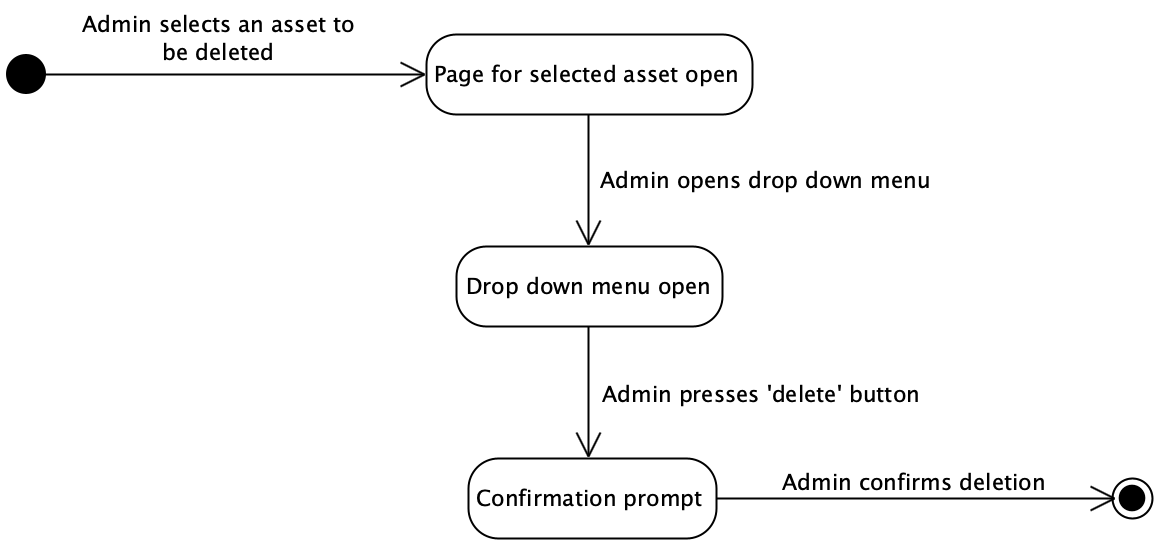
\includegraphics[width=1.0\textwidth]{figures/RemoveAsset.png}
    \caption{Use case diagram for removing an asset.}
    \label{fig:UseCaseRemoveAsset}
\end{figure}

%%%%%%%%%%%%%%%%%%%%%%%%%%%%%%%%%%%%%%

\begin{use_case}[H]
    \hrule
    \vskip 0.3cm
    \Large
    \begin{center}
    
        \textbf{Adding a tag}
        
    \end{center}
    \vskip 0.1cm
    \hrule
    \vskip 0.2cm
    \normalsize
    
    \textbf{Use Case:} The process of adding a \textit{tag} to the system is initiated by an \textit{admin} in one of two ways. The first is by going to the 'tag' page, typing in a \textit{tag} name, and, if the \textit{tag} does not exist, pressing 'add'. The second is by simply pressing 'add tag' on the 'tag' page. The \textit{admin} is then taken to a new page, where he/she can set the label of the \textit{tag}, add new \textit{fields} and change the color of the \textit{tag}. If the \textit{admin} added the \textit{tag} using the first way, the label is already set. If the \textit{admin} chooses to add a new \textit{field} to the \textit{tag}, a new window pops up on top of the page. This window presents a few options to the \textit{admin}.\\
    The \textit{field} has a label, a list of types (short text, text box, number, checkbox), a default value for the \textit{field}, and a checkbox to determine rather or not the \textit{field} is required. The list of types specifies and restricts the input type.\\
    The \textit{admin} can also set the \textit{parent tag}, from which the \textit{tag} inherits its color. The color can be change, if it needs to differ from the color of the \textit{parent tag}.
    
    \vskip 0.2cm
    
    \textbf{Objects:} Admin, Tag, Field, Log
    
    \vskip 0.2cm
    
    \textbf{Functions:} Add tag, Add field
    
    \vskip 0.4cm
    \hrule
    \vskip 0.2cm
    \caption{Adding a tag} \label{use_case:adding_a_tag}
\end{use_case}

%%%%%%%%%%%%%%%%%%%%%%%%%%%%%%%%%%%%%%

\begin{use_case}[H]
    \hrule
    \vskip 0.3cm
    \Large
    \begin{center}
    
        \textbf{Editing a tag}
        
    \end{center}
    \vskip 0.1cm
    \hrule
    \vskip 0.2cm
    \normalsize
    
    \textbf{Use Case:} An \textit{admin} goes to the 'tag' page, where the \textit{admin} is presented with a list of tags. Next to every entry a pencil symbol is located. When the symbol is pressed, the \textit{admin} is taken to a page very similar to the 'add tag' page, but where the \textit{fields} of the \textit{tag} are already added. The \textit{admin} can then add or remove \textit{fields}, rename the \textit{tag} and change the color. When the wanted changes have been made, the \textit{admin} presses save and the tag is saved.
    
    \vskip 0.2cm
    
    \textbf{Objects:} Admin, Tag, Field, Log
    
    \vskip 0.2cm
    
    \textbf{Functions:} Edit tag, Add field, Edit field, Remove field
    
    \vskip 0.4cm
    \hrule
    \vskip 0.2cm
    \caption{Editing a tag} \label{use_case:editing_a_tag}
\end{use_case}

%%%%%%%%%%%%%%%%%%%%%%%%%%%%%%%%%%%%%%

\begin{use_case}[H]
    \hrule
    \vskip 0.3cm
    \Large
    \begin{center}
    
        \textbf{Removing a tag}
        
    \end{center}
    \vskip 0.1cm
    \hrule
    \vskip 0.2cm
    \normalsize
    
    \textbf{Use Case:} A \textit{tag} can be removed from the 'tag' page by an \textit{admin}. On the 'tag' page, a list of tags is shown and beside every entry in the list is a trashcan, which prompts the \textit{admin} when pressed. If accepted, the \textit{tag} and all its relations to assets are removed from the system.
    
    \vskip 0.2cm
    
    \textbf{Objects:} Admin, Tag, Log
    
    \vskip 0.2cm
    
    \textbf{Functions:} Remove tag
    
    \vskip 0.4cm
    \hrule
    \vskip 0.2cm
    \caption{Removing a tag} \label{use_case:removing_a_tag}
\end{use_case}

\begin{figure}[H]
    \centering
    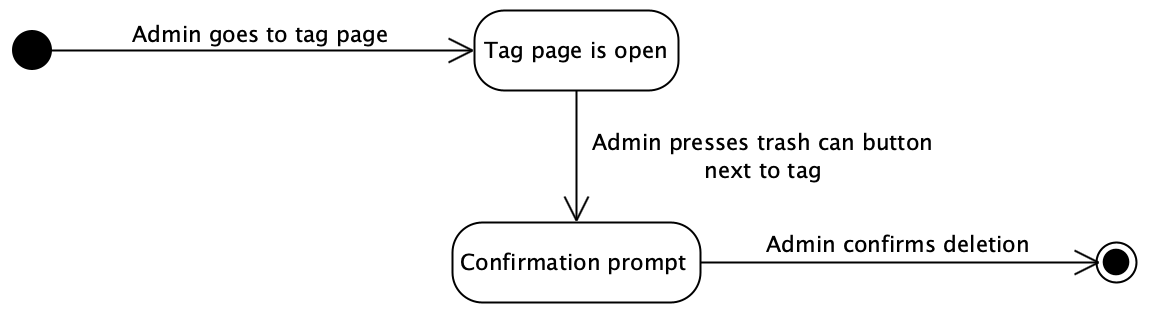
\includegraphics[width=1.0\textwidth]{figures/RemoveTag.png}
    \caption{Use case diagram for removing a tag.}
    \label{fig:UseCaseRemoveTag}
\end{figure}

%%%%%%%%%%%%%%%%%%%%%%%%%%%%%%%%%%%%%%

\begin{use_case}[H]
    \hrule
    \vskip 0.3cm
    \Large
    \begin{center}
    
        \textbf{Adding a comment to an asset}
        
    \end{center}
    \vskip 0.1cm
    \hrule
    \vskip 0.2cm
    \normalsize
    
    \textbf{Use Case:} Adding a \textit{comment} is initiated by either a \textit{viewer} or an \textit{admin} going to a specific asset and pressing the 'add comment' button. The \textit{user} (\textit{viewer} or \textit{admin}) is then presented to a text box, where they can type in their \textit{comment}. When the \textit{user} has finished the comment, he/she presses the 'add' button and the \textit{comment} is attached to the \textit{asset}, ending the use case.
    
    \vskip 0.2cm
    
    \textbf{Objects:} Admin, Viewer, Comment, Asset, Log
    
    \vskip 0.2cm
    
    \textbf{Functions:} Add comment
    
    \vskip 0.4cm
    \hrule
    \vskip 0.2cm
    \caption{Adding a comment to an asset} \label{use_case:adding_a_comment_to_an_asset}
\end{use_case}

\begin{figure}[H]
    \centering
    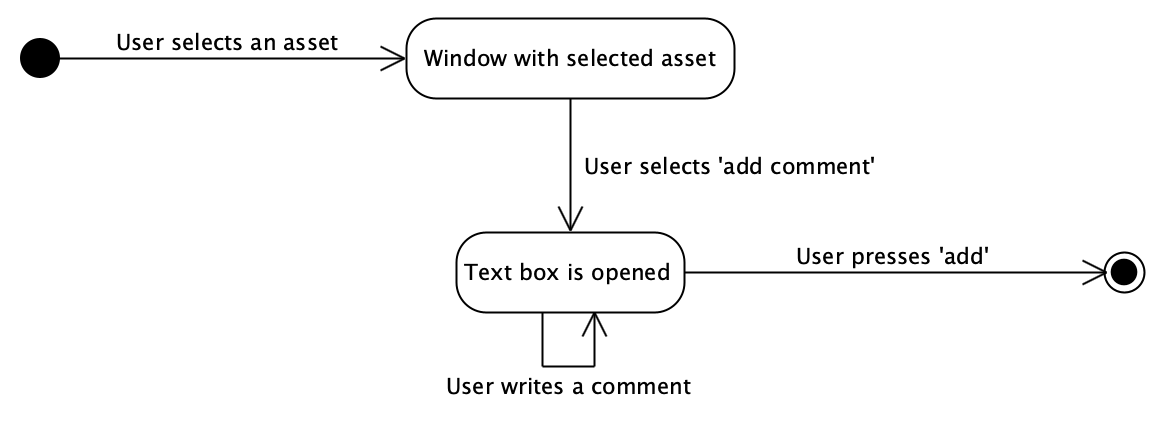
\includegraphics[width=1.0\textwidth]{figures/AddComment.png}
    \caption{Use case diagram for adding a comment.}
    \label{fig:UseCaseAddComment}
\end{figure}

%%%%%%%%%%%%%%%%%%%%%%%%%%%%%%%%%%%%%%

\begin{use_case}[H]
    \hrule
    \vskip 0.3cm
    \Large
    \begin{center}
    
        \textbf{Adding a department}
        
    \end{center}
    \vskip 0.1cm
    \hrule
    \vskip 0.2cm
    \normalsize
    
    \textbf{Use Case:} Adding a \textit{department} to the system is initiated by an \textit{admin} by pressing the dropdown-menu with the current \textit{department} and pressing the last element in the menu named 'add new department'. An input field then pops up in a new window and the \textit{admin} can type in the name of the new \textit{department}.
    
    \vskip 0.2cm
    
    \textbf{Objects:} Admin, Department, Log
    
    \vskip 0.2cm
    
    \textbf{Functions:} Add department
    
    \vskip 0.4cm
    \hrule
    \vskip 0.2cm
    \caption{Adding a department} \label{use_case:adding_a_department}
\end{use_case}

\begin{figure}[H]
    \centering
    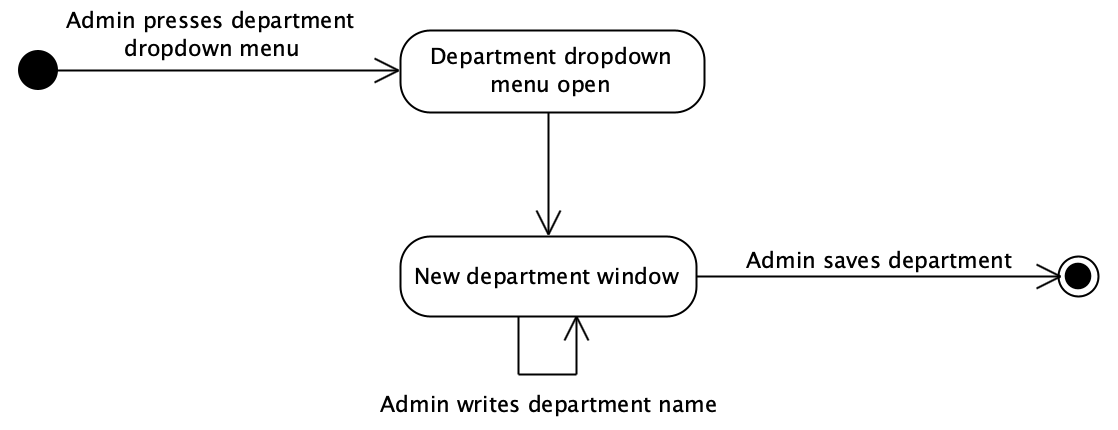
\includegraphics[width=1.0\textwidth]{figures/AddDepartment.png}
    \caption{Use case diagram for adding a department.}
    \label{fig:UseCaseAddDepartment}
\end{figure}

%%%%%%%%%%%%%%%%%%%%%%%%%%%%%%%%%%%%%

\begin{use_case}[H]
    \hrule
    \vskip 0.3cm
    \Large
    \begin{center}
    
        \textbf{Renaming a department}
        
    \end{center}
    \vskip 0.1cm
    \hrule
    \vskip 0.2cm
    \normalsize
    
    \textbf{Use Case:} If a \textit{department} has been named incorrectly, the \textit{admin} can press a pencil symbol besides each \textit{department} name in the dropdown-menu, and the same window as for adding a new \textit{department} pops up, but with the department name already filled in. The \textit{admin} then changes the name, presses 'save', and the \textit{department} is renamed, ending the use case.
    
    \vskip 0.2cm
    
    \textbf{Objects:} Admin, Department, Log
    
    \vskip 0.2cm
    
    \textbf{Functions:} Rename department
    
    \vskip 0.4cm
    \hrule
    \vskip 0.2cm
    \caption{Renaming a department} \label{use_case:renaming_a_department}
\end{use_case}

\begin{figure}[H]
    \centering
    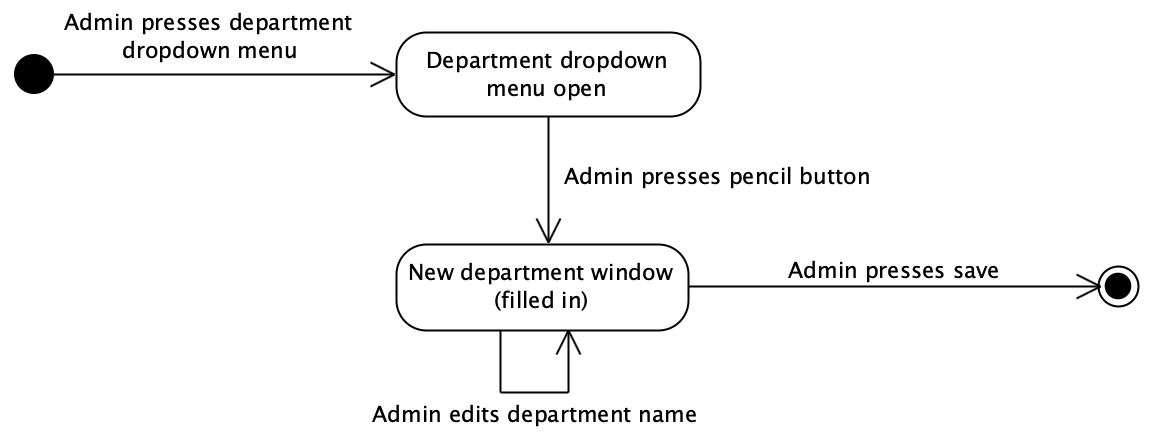
\includegraphics[width=1.0\textwidth]{figures/EditDepartment.png}
    \caption{Use case diagram for renaming a department.}
    \label{fig:UseCaseRenameDepartment}
\end{figure}

%%%%%%%%%%%%%%%%%%%%%%%%%%%%%%%%%%%%%%%%

\begin{use_case}[H]
    \hrule
    \vskip 0.3cm
    \Large
    \begin{center}
    
        \textbf{Deleting a department}
        
    \end{center}
    \vskip 0.1cm
    \hrule
    \vskip 0.2cm
    \normalsize
    
    \textbf{Use Case:} If a \textit{department} is no longer needed, the \textit{admin} can press the trashcan besides the pencil symbol in the dropdown-menu next to the given \textit{department}. The \textit{admin} is then prompted with a confirmation message and, where the \textit{admin} can accept the deletion of the department, ending the use case.
    
    \vskip 0.2cm
    
    \textbf{Objects:} Admin, Department, Log
    
    \vskip 0.2cm
    
    \textbf{Functions:} Delete department
    
    \vskip 0.4cm
    \hrule
    \vskip 0.2cm
    \caption{Deleting a department} \label{use_case:deleting_a_department}
\end{use_case}

\begin{figure}[H]
    \centering
    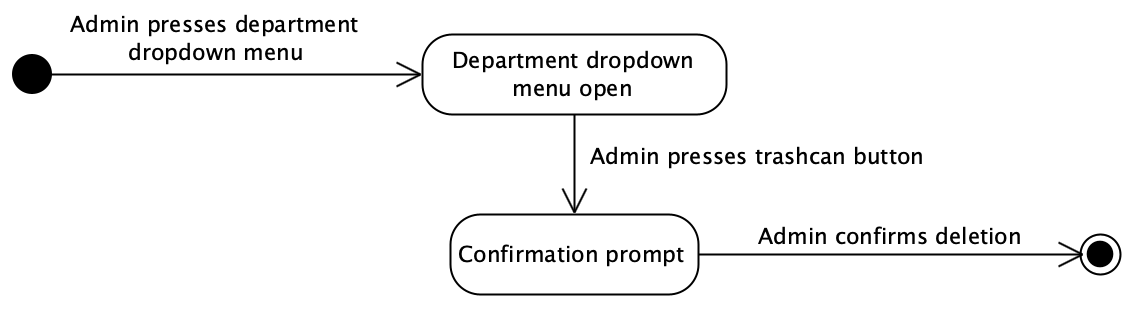
\includegraphics[width=1.0\textwidth]{figures/DeleteDepartment.png}
    \caption{Use case diagram for deleting a department.}
    \label{fig:UseCaseDeleteDepartment}
\end{figure}

%%%%%%%%%%%%%%%%%%%%%%%%%%%%%%%%%%%%%%%%

\begin{use_case}[H]
    \hrule
    \vskip 0.3cm
    \Large
    \begin{center}
    
        \textbf{Searching through assets}
        
    \end{center}
    \vskip 0.1cm
    \hrule
    \vskip 0.2cm
    \normalsize
    
    \textbf{Use Case:} Both the \textit{admin} and the \textit{viewer} can search through the assets in the system, by going to the 'asset' page, where a list of assets are presented to the \textit{user}, and entering a search query. This search query can be either tags or plain text. The system then returns a list of assets matching the search query, within the selected department, and the \textit{user} can go to a specific asset page or, if the \textit{user} is an \textit{admin}, print out the list.
    
    \vskip 0.2cm
    
    \textbf{Objects:} Admin, Viewer, Tag, Asset, Field, Department
    
    \vskip 0.2cm
    
    \textbf{Functions:} Search asset
    
    \vskip 0.4cm
    \hrule
    \vskip 0.2cm
    \caption{Searching through assets} \label{use_case:searching_through_assets}
\end{use_case}

\begin{figure}[H]
    \centering
    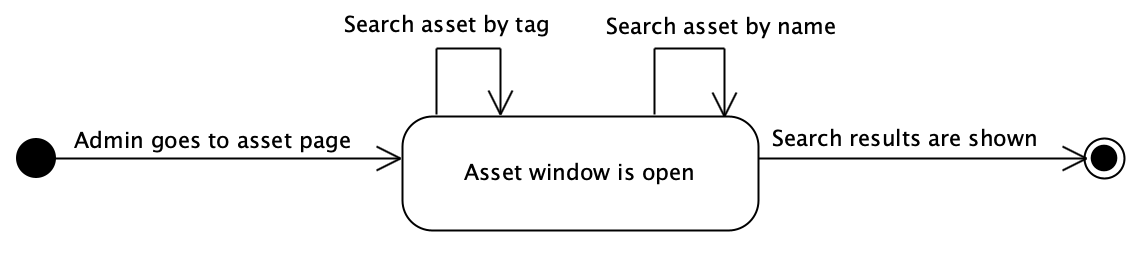
\includegraphics[width=1.0\textwidth]{figures/SearchAssets.png}
    \caption{Use case diagram for searching through the assets.}
    \label{fig:UseCaseSearchAssets}
\end{figure}

%%%%%%%%%%%%%%%%%%%%%%%%%%%%%%%%%%%%%%%%

\begin{use_case}[H]
    \hrule
    \vskip 0.3cm
    \Large
    \begin{center}
    
        \textbf{Printing a report}
        
    \end{center}
    \vskip 0.1cm
    \hrule
    \vskip 0.2cm
    \normalsize
    
    \textbf{Use Case:} When an \textit{admin} wants to print out a report, he/she goes to the 'asset' page and presses 'print report'. If the \textit{admin} only wants a limited set of the \textit{assets} to be printed in the report, he/she can search through the \textit{assets} first and then press 'print report'. This will create a report only containing the search results.
    
    \vskip 0.2cm
    
    \textbf{Objects:} Admin, Asset, Tag, Field
    
    \vskip 0.2cm
    
    \textbf{Functions:} Printing report, Searching through assets
    
    \vskip 0.4cm
    \hrule
    \vskip 0.2cm
    \caption{Printing a report} \label{use_case:printing_a_report}
\end{use_case}

\begin{figure}[H]
    \centering
    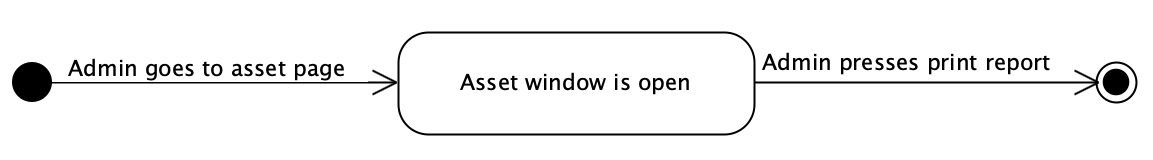
\includegraphics[width=1.0\textwidth]{figures/PrintReport.png}
    \caption{Use case diagram for printing a report.}
    \label{fig:UseCasePrintReport}
\end{figure}

%%%%%%%%%%%%%%%%%%%%%%%%%%%%%%%%%%%%%%%%%

\begin{use_case}[H]
    \hrule
    \vskip 0.3cm
    \Large
    \begin{center}
    
        \textbf{Searching through the log}
        
    \end{center}
    \vskip 0.1cm
    \hrule
    \vskip 0.2cm
    \normalsize
    
    \textbf{Use Case:} Searching through the log is initiated by the \textit{admin}, when he/she goes to the 'log' page and enters a search query. At the 'log' page, the \textit{admin} is presented with a list of log entries and can search through them with a search query containing plain text. The list is then updated to show the corresponding entries and the admin can print out the results.
    
    \vskip 0.2cm
    
    \textbf{Objects:} Admin, Log
    
    \vskip 0.2cm
    
    \textbf{Functions:} Search log
    
    \vskip 0.4cm
    \hrule
    \vskip 0.2cm
    \caption{Searching through the log} \label{use_case:searching_through_the_log}
\end{use_case}

\begin{figure}[H]
    \centering
    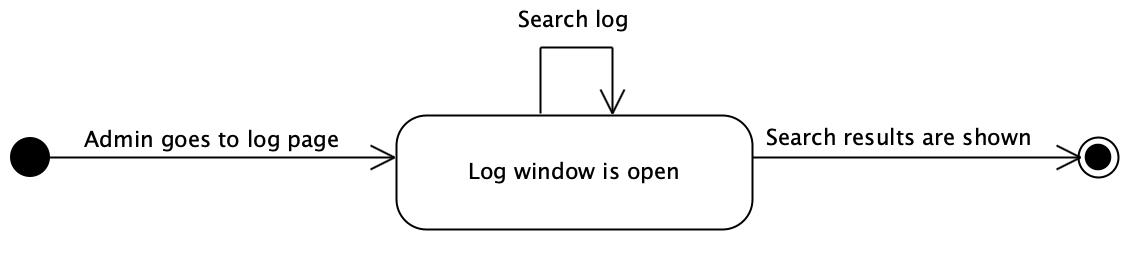
\includegraphics[width=1.0\textwidth]{figures/SearchLog.png}
    \caption{Use case diagram for searching til log.}
    \label{fig:UseCaseSearchLog}
\end{figure}

%%%%%%%%%%%%%%%%%%%%%%%%%%%%%%%%%%%%%%

\begin{use_case}[H]
    \hrule
    \vskip 0.3cm
    \Large
    \begin{center}
    
        \textbf{Printing the log}
        
    \end{center}
    \vskip 0.1cm
    \hrule
    \vskip 0.2cm
    \normalsize
    
    \textbf{Use Case:} When an \textit{admin} wants to print out the log, he/she goes to the 'log' page and presses 'print log'. If the \textit{admin} only wants a limited set of the log entries to be printed, he/she can search through the log first and then press 'print log'. This will create a list only containing the search results.
    
    \vskip 0.2cm
    
    \textbf{Objects:} Admin, Asset, Tag, Field
    
    \vskip 0.2cm
    
    \textbf{Functions:} Printing the log, Searching through the log
    
    \vskip 0.4cm
    \hrule
    \vskip 0.2cm
    \caption{Printing the log} \label{use_case:printing_the_log}
\end{use_case}

\begin{figure}[H]
    \centering
    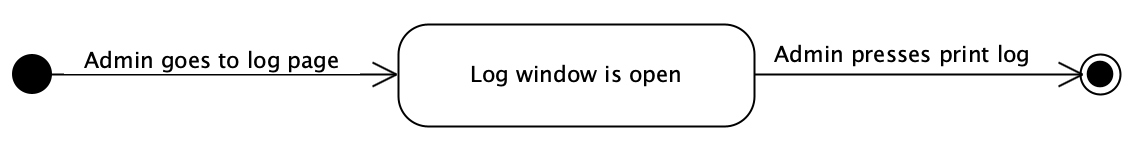
\includegraphics[width=1.0\textwidth]{figures/PrintLog.png}
    \caption{Use case diagram for printing til log.}
    \label{fig:UseCasePrintLog}
\end{figure}
\section{Actor Table}\label{sc:actortable}

The actors are involved with different use cases, as described in table \ref{tab:actortable}

\begin{table}[H]
    \centering
    \begin{tabular}{|l|c|c|}
        \hline
         & \textbf{Admin} & \textbf{Viewer}  \\
        \hline
        Adding an asset & \textbf{X} & \\
        \hline
        Editing an asset & \textbf{X} & \\
        \hline
        Adding a tag & \textbf{X} & \\
        \hline
        Editing a tag & \textbf{X} & \\
        \hline
        Adding a comment & \textbf{X} & \textbf{X} \\
        \hline
        Adding a department & \textbf{X} & \\
        \hline
        Renaming a department & \textbf{X} & \\
        \hline
        Searching for an asset & \textbf{X} & \textbf{X} \\
        \hline
        Printing a report & \textbf{X} & \\
        \hline
        Printing the log & \textbf{X} & \\
        \hline
        Searching the log & \textbf{X} & \\
        \hline
        Removing an asset or a tag & \textbf{X} & \\
        \hline
        
    \end{tabular}
    \caption{Actor table showing which actors are involved in the different use cases, described in section \ref{sc:usecases}. An actors involvement in a particular use case is marked by an \textbf{X} in the table.}
    \label{tab:actortable}
\end{table}

As seen in the actor table (table \ref{tab:actortable}) the \textit{admin} is involved in all the use cases, while the \textit{viewer} is only involved in two. This reflects the fact that the program is primarily intended for the \textit{admin}, as they are the ones managing their asserts, while the \textit{viewer} is only given access to view and comment on the assets in the system. 

\section{Functions}\label{sc:functions}

This section will present the functions in the system. Table \ref{tab:functions} shows all the top-level functions that the system will be able to perform. All the tables describing functions have columns with the name of the function, the complexity and the type of function.

\begin{table}[H]
\centering
%\resizebox{\textwidth}{!}{%
    \begin{tabular}{|l|l|l|}
        \hline
        \textbf{Function} & \textbf{Complexity} & \textbf{Type} \\
        \hline
        \hline
        Add Asset & Complex & Update\\
        \hline
        Remove Asset & Medium & Update\\
        \hline
        Edit Asset & Complex & Update\\
        \hline
        Search Asset & Medium & Compute/Read\\
        \hline
        View Asset & Simple & Read\\
        \hline
        Add Template & Complex & Update\\
        \hline
        Remove Template & Medium & Update\\
        \hline
        Edit Template & Complex & Update\\
        \hline
        Add Tag & Simple & Update\\
        \hline
        Remove Tag & Medium & Update\\
        \hline
        Rename Tag & Simple & Update\\
        \hline
        Tag Asset & Simple & Update\\
        \hline
        Untag Asset & Simple & Update\\
        \hline
        Authenticate User & Simple & Read\\
        \hline
        Check access level & Simple & Read\\
        \hline
        Export report & Complex & Compute/Read\\
        \hline
    
    \end{tabular}
%}
\caption{Table showing all the different top-level functions as well as their complexity and type.}\label{tab:functions}
\end{table}

\par

Table \ref{tab:functions} contains several functions rated complex. These functions have been divided into several smaller functions, with a lower complexity.
% Beskriver hvorfor det er gjort, ved ikke om det skal med, men det er god fyldertekst
This is done in order to divide the complex problems, into smaller problems, which are easier to implement. 
 
\begin{center}
    \textbf{Adding an asset}
\end{center}

% Add asset table
\begin{table}[H]
\centering
%\resizebox{\textwidth}{!}
\caption{Table showing the different functions involved in adding an asset along with their complexity and type.}\label{tab:AddAssetFunctions}
\end{table}

\par

\begin{center}
    \textbf{Editing an asset}
\end{center}

% Edit Asset Table
\begin{table}[H]
\centering
%\resizebox{\textwidth}{!}
\caption{Table showing the different functions involved in editing an asset along with their complexity and type.}\label{tab:EditAssetFunctions}
\end{table}

\par

\begin{center}
    \textbf{Adding a template}
\end{center}

% Add template table 
\begin{table}[H]
\centering
%\resizebox{\textwidth}{!}
\caption{Table showing the different functions involved in adding a template along with their complexity and type.}\label{tab:AddTemplateFunctions}
\end{table}

\par

\begin{center}
    \textbf{Editing a template}
\end{center}

% Edit template table
\begin{table}[H]
\centering
%\resizebox{\textwidth}{!}
\caption{Table showing the different functions involved in editing a template along with their complexity and type.}\label{tab:EditTemplateFunctions}
\end{table}

\par

\begin{center}
    \textbf{Exporting a report}
\end{center}

% Export report table
\begin{table}[H]
\centering
%\resizebox{\textwidth}{!}
\caption{Table showing the different functions involved in exporting a report along with their complexity and type.}\label{tab:ExportReportFunctions}
\end{table}
\section{PACT analysis}\label{sc:PACT}


\textbf{People}:
%(Physiological differences, Psychological differences, Social differences, Domain Expertise)
\begin{itemize}
    \item Morten (IT)
    \item Kasper (IT)
    \item Employees at the zoo
\end{itemize}

\par
No physiological, physiological or social differences to speak of. Morten and Kasper are both IT people, which means they are used to working with computers. However, they have requested the interface to be minimalistic and easy to use, which means most people should be able to use it.
The other employees at the zoo have experience with other computer-based systems through their work.
\par

\textbf{Activities}: \\
%(Purpose of activities to be supported by the system, Temporal aspects, Collaboration, Complexity, Safety criticality, Nature of system content) \\
The system will support registration of assets, and helping users keep track of them. The IT-department adds, edits, updates and removes assets from the system and exports list of assets. They also log changes to the assets and keep track of the assets. On occasion they want a specific asset, which should be easily available to them.
The rest of the employees only use the system to see assets and their current state.
\par

\textbf{Context}: \\
%(Physical, Social, Organizational) \\
The system will be used at Aalborg Zoo, primarily on a desktop or laptop located in the office of the IT department. The laptops might be moved around the premise of the zoo. The software does not contain any elements geared towards any social aspects.
Within Aalborg Zoo the program is developed specifically for the IT department.
\par
 
\textbf{Technology}:
%(That could support users in the domain)
\begin{itemize}
    \item Computer
    \item Barcode scanner
    \item Screen
    \item Mouse
    \item Keyboard
    \item Internet
    \item Database
    \item Active Directory (AD)
\end{itemize}

\section{Scope of the Application}\label{sc:scope}
The main purpose of the system is to assist in the management of assets at Aalborg Zoo, specifically their IT department. As such the application should be able to help keep track of the different assets and their information, so the admins know where their assets are and what state they are in. 
\par
The admin will be able to add, edit and remove assets, using tags to provide flexible information about the asset. They will also be able search through existing assets using tags and print out a log of assets, with all their information. This will allow them too keep an overview of their assets. 
\par
Any other users of the system (viewers) are able to search through the assets and comment on assets if they have relevant information to share. The admin and other viewers can then view these comments. 
\par
This results in a flexible system where the admin has control while the viewer can still look through assets they may need to borrow and give feedback on things they have previously borrowed. 
% Design...
\chapter{Design and implementation}
This chapter will go through the processes of designing and implementing the system for Aalborg Zoo, as well as discussing the thoughts behind the coding and design.

\section{Architectural design}
Upon development of the program, more components, and subsystems have been added to the system structure. The system has been split into smaller parts to get a better understanding of the components of the system, a more detailed class diagram have been made. These components will be discussed in the following section.

\subsection{Component design}
This section will focus on explaining the different components of the program, and their relations. As well as describing the functions of the individual sub-systems, and their components.

\subsubsection{Fields}\todo[Inline]{Better name}
\begin{figure}[H]
    \centering
    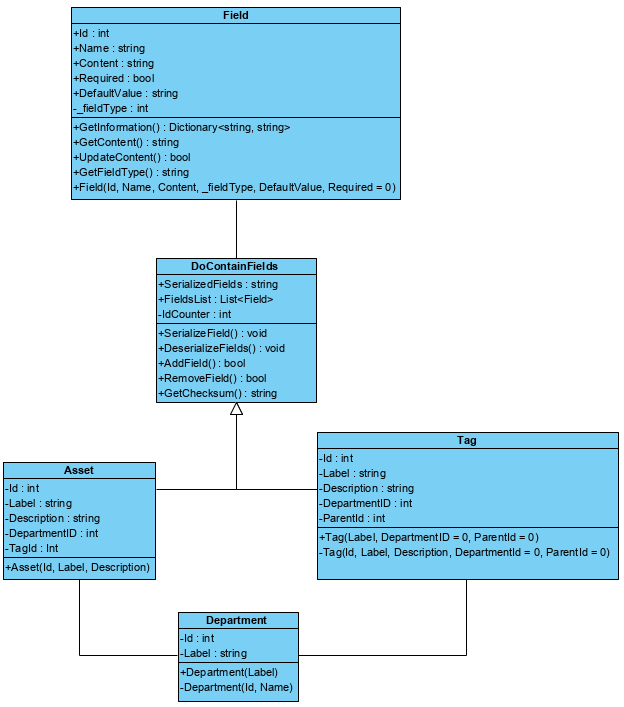
\includegraphics{figures/FieldsComponent.PNG}
    \caption{Componentdiagram for the Field Component}
    \label{fig:FieldsComponent}\todo[Inline]{Upload nyt diagram, med abstrakt DoContainFields}
\end{figure}
This components function is to describe the general in formations needed for the two classes containing instances of \textit{fields}. The classes which needs \textit{fields} are \textit{Asset} and \textit{Tag}, both of these aggregates functions and variables from \textit{DoContainFields}. The functions aggregated are functions related to controlling fields and their behavior on the aggregating classes. As both \textit{Tag} and \textit{Asset} needs to be able to utilize the same functionalities when handling \textit{Fields} and serializing these. 
\par
The serilization of the fields is done to JSON. The reason for choosing to utilize JSON is that MYSQL and other newer database versions, can index JSON so it counts as virtual rows within the database. These virtual rows enables searching the JSON fields, with ordinary SQL queries.



\section{UI design}
Model-View-Viewmodel (MVVM) design pattern
\section{Implementation}
% Conclusion
\chapter{Conclusion}\label{ch:conclusion}




%%% End of document
\printbibliography[heading=bibintoc]
\label{bib:mybiblio}
\appendix
%\chapter{Appendix A name}\label{ch:appAlabel}
Here is the first appendix

\end{document}
